%% International Journal of Computational Intelligence Systems ---
%%%%%%%%%%%%%%%%%%%%%%%%%%%%%%%%%%%%%%%%%%%%%%%%%%%%%%%%%%%%%%%%%%%%%%%%%%%
\documentclass[11pt,twoside]{article}
\usepackage{ijcis}
%--------------------- ADDITIONAL PACKAGES HERE ---------------------------
\usepackage{lscape}
\usepackage{pdflscape}
\usepackage{setspace}
\usepackage{afterpage}
\usepackage{alltt}
\usepackage{epstopdf}
%--------------------------------------------------------------------------
%
\def\labart{yourLabel}      % put a label from your choice here
%\Vol{1}                    % number of the Volume
%\Issue{1}                  % number of the issue
%\Month{January}            % month
%\Year{2008}                % year
%\received{...}
%\revised{...}
%
%---------------------------------------------------------------------------
\thispagestyle{empty}
%%------------------------- YOUR HEADINGS HERE -----------------------------
% Author's initials of first names+last names
\shortauthors{Pablo Cingolani, Jes\'us Alcal\'a-Fdez}
% Short title
\shorttitle{jFuzzyLogic}
%---------------------------------------------------------------------------
%
%---------------------- YOUR TITLE ----------------------------------------
\title{jFuzzyLogic: a Java Library to Design Fuzzy Logic Controllers According to the Standard for Fuzzy Control Programming}
%-------------------------- AUTHOR'S NAMES ----------------------------------
\author{%
Pablo Cingolani\,\up{1},
%\author{
Jes\'us Alcal\'a-Fdez\,\up{2}
}
%----------------------------- ADDRESSES ----------------------------------
\addresses\address{%
\\ \vspace*{0.05truein}
\up{2}
Department of Computer Science and Artificial Intelligence,\\
Research Center on Information and Communications Technology (CITIC-UGR),\\
University of Granada, Granada, 18071, Spain
\\ \vspace*{0.04truein}
E-mail: jalcala@decsai.ugr.es
}
%---------------------------------------------------------------------------
\pagestyle{myheadings}
\begin{document}
\label{\labart-FirstPage}

\maketitle
%-------------------------- ABSTRACT ---------------------------------------
\abstracts{%
Fuzzy Logic Controllers are a specific model of Fuzzy Rule Based Systems suitable for engineering applications for which classic control strategies do not achieve good results or for when it is too difficult to obtain a mathematical model. Recently, the International Electrotechnical Commission has published a standard for fuzzy control programming in part 7 of the IEC 61131 norm in order to offer a well defined common understanding of the basic means with which to integrate fuzzy control applications in control systems. In this paper, we introduce an open source Java library called jFuzzyLogic which offers a fully functional and complete implementation of a fuzzy inference system according to this standard, providing a programming interface and Eclipse plugin to easily write and test code for fuzzy control applications. A case study is given to illustrate the use of jFuzzyLogic.
}
\par\bigskip\par
%-------------------------- KEYWORDS ---------------------------------------
\keywords{Fuzzy Logic Control, Fuzzy Control Language, Fuzzy Logic, IEC 61131-7, Open Source Software, Java Library}

\vspace*{10pt}\textlineskip
%-------------------------- BEGIN BODY OF TEXT -----------------------------
\begin{multicols}{2}

\section{Introduction}
Expert Control is a field of Artificial Intelligence that has become a research topic in the domain of system control. 

Fuzzy Logic Control~\cite{Lee90,DHR93,Bon94} is one of the topics within Expert Control which allows us to enhance the capabilities of industrial automation. It is suitable for engineering applications in which classical control strategies do not achieve good results or when it is too difficult to obtain a mathematical model. Fuzzy Logic Controllers (FLCs) are a specific model of Fuzzy Rule Based Systems (FRBSs) that provide a tool which can convert the linguistic control strategy based on expert knowledge into an automatic control strategy. They usually have two characteristics: the need for human operator experience, and a strong non-linearity. Nowadays, there are many real-world applications of FLCs such as mobile robot navigation \cite{EH2010,JCh2011}, air conditioning controllers \cite{Alc09,Cho11}, domotic control\cite{Cha12,AL05}, and industrial applications\cite{Otero2008,Demir12,ZG2012}.

FLCs are powerful when solving a wide range of problems, but their implementation requires a certain programming expertise. In the last few years, many fuzzy logic software tools have been developed to minimise this requirement. Although many of them are commercially distributed, for example MATLAB Fuzzy logic toolbox\fnm{a}\fnt{a}{\url{http://www.mathworks.com}}, a few are available as open source software. Open source tools can play an important role as is pointed out in~\cite{Sonnenburg07}. 

Recently, the International Electrotechnical Commission published the 61131 norm (IEC 61131)~\cite{IEC}, which has become well known for defining the Programmable Controller Languages (PLC) and is commonly used in industrial applications. In part 7 (IEC 61131-7) of this norm Fuzzy Control Language (FCL) is defined, offering common understanding of the basic means with which to integrate fuzzy control applications in control systems and providing a common language with which to exchange portable fuzzy control programs among different platforms. This standard has a world-wide diffusion and is independent of systems manufactures, which has many advantages: easy migration to and from several hardware platforms from different manufacturers; protection of investment at both the training and application-level; conformity with the requirements of the Machinery Directive EN60204; and reusability of the developed application.

In this paper, we present an open source Java library called jFuzzyLogic\fnm{b}\fnt{b}{\url{http://jfuzzylogic.sourceforge.net}} which allows us to design and to develop FLCs following the standard for FCL. jFuzzyLogic offers a fully functional and complete implementation of a fuzzy inference system (FIS), and provides a programming interface (API) and an Eclipse plugin in order to make it easier to write and test FCL code. This library brings the benefits of open source software and standardization to the fuzzy systems community, which has several advantages:
\begin{itemize}
	\item Standardization reduces programming work. This library contains the basic programming elements for the standard IEC 61131-7, removing the need for developers to attend to boiler plate programming tasks.
	\item This library extends the range of possible users applying FLCs. This provides a complete implementation of FIS following the standard for FCL, reducing the level of knowledge and experience in fuzzy logic control required of researchers. As a result researchers with less knowledge will be able to successfully apply FLCs to their problems when using this library.
	\item The strict object-oriented approach, together with the modular design used for this library, allows developers to extend it easily.
	\item jFuzzyLogic follows a platform-independent approach, which enables it to be developed and run on any hardware and operating system configuration that supports Java.
\end{itemize}

This paper is arranged as follows. The next section introduces the basic definitions of the FLCs and the published PLCs in the IEC 61131 norm. In Section~\ref{sec:stu} we review some non-commercial fuzzy softwares and the main benefits that the jFuzzyLogic offers with respect to other softwares. Section~\ref{sec:jFu} presents jFuzzyLogic: its main features and components. In Section~\ref{sec:cas}, a FLC is used in order to illustrate how jFuzzyLogic can be used in a control application. Finally, Section~\ref{sec:con} draws some conclusions and indicates future work.

\section{Preliminaries}
In this section, we first introduce the basic definitions of the FLCs, and then we present the published PLCs by the IEC 61131 norm.

\subsection{Fuzzy logic controller}
FLCs, as initiated by Mamdani and Assilian~\cite{Mamdani1974,MA1975}, are currently considered to be one of the most important applications of the fuzzy set theory proposed by Zadeh~\cite{Zadeh1965}. This theory is based on the notion of the fuzzy set as a generalization of the ordinary set characterized by a membership function $\mu$ that takes values from the interval [0, 1] representing degrees of membership in the set. FLCs typically define a non-linear mapping from the system's state space to the control space. Thus, it is possible to consider the output of a FLC as a non-linear control surface reflecting the process of the operator's prior knowledge.

A FLC is a kind of FRBS which is composed of: A Knowledge Base (KB) that comprises the information used by the expert operator in the form of linguistic control rules; a Fuzzification Interface, which transforms the crisp values of the input variables into fuzzy sets that will be used in the fuzzy inference process; an Inference System that uses the fuzzy values from the Fuzzification Interface and the information from the KB to perform the reasoning process; and the Defuzzification Interface, which takes the fuzzy action from the inference process and translates it into crisp values for the control variables. Figure~\ref{f:FLC} shows the generic structure of a FLC.

\vspace*{9pt}
\centerline{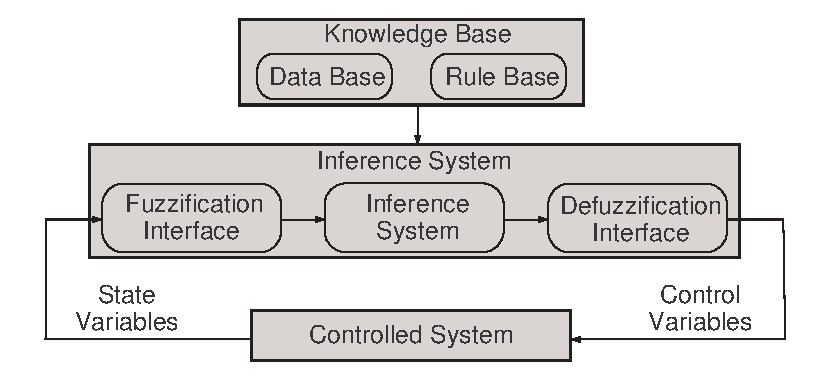
\includegraphics[width=3.15in]{./figs/FRBS-mam.eps}}
\vspace*{3pt}
\fcaption{Generic structure of a FLC.}\label{f:FLC}
\vspace*{5pt}

The KB encodes the expert knowledge by means of a set of fuzzy control rules. A fuzzy control rule is a conditional statement in which the antecedent is a condition in its application domain, the consequent is a control action to be applied in the controlled system and both, antecedent and consequent, are associated with fuzzy concepts; that is, linguistic terms. The KB includes two components: the Data Base (DB) and the Rule Base (RB). The DB contains the definitions of the linguistic labels; that is, the membership functions for the fuzzy sets. The RB is a collection of fuzzy control rules, comprised by the linguistic labels, representing the expert knowledge of the controlled system.

The Fuzzification Interface establishes a mapping between each crisp value of the input variable and a fuzzy set defined in the universe of the corresponding variable. This interface works as follows:

\vspace*{5pt}
$A'$ = $F(x_0)$
\vspace*{5pt}

\noindent where $x_0$ is a crisp value defined in the input universe $U$, $A'$ is a fuzzy set defined in the same universe and $F$ is a fuzzifier operator.

The Inference System is based on the application of the Generalized Modus Ponens, an extension of the classical Modus Ponens, proposed by Zadeh in which: 

\vspace*{5pt}
\begin{tabular}{l}
If $X$ is $A$ then $Y$ is $B$\\
$X$ is $A'$\\
\hline
$Y$ is $B'$\\
\end{tabular}
\vspace*{5pt}

\noindent where $X$ and $Y$ are linguistic variables, $A$ and $B$ are fuzzy sets, and $B'$ is the output fuzzy set inferred. To do this, the system firstly obtains the degree of matching of each rule by applying a conjunctive operator (called an aggregation operator in the IEC-61131-7 norm), and then infers the output fuzzy sets by means of a fuzzy implication operator (called activation operator in the IEC-61131-7 norm). The Inference System produces the same amount of output fuzzy sets as the number of rules collected in the KB. These groups of fuzzy sets are aggregated by an aggregation operator (called an accumulation operator in the IEC-61131-7 norm), but they must be transformed into crisp values for the control variables. This is the purpose of the Defuzzification Interface. There are two types of defuzzification methods~\cite{Wan94,CHP97} depending on the way in which the individual fuzzy sets $B'$ are aggregated:
\begin{itemize}
\item Mode A: Aggregation First, Defuzzification After. The Defuzzification Interface performs the aggregation of the individual fuzzy sets inferred, $B'$, to obtain the final output fuzzy set. Usually, the aggregation operator is the minimum or the maximum.
\item Mode B: Defuzzification First, Aggregation After. This avoids the computation of the final fuzzy set by considering the contribution of each rule output individually, obtaining the final control action by taking a calculation (an average, a weighted sum or a selection of one of them) of a concrete crisp characteristic value associated with each of them.
\end{itemize}
More complete information on FLCs can be found in~\cite{Lee90,DHR93,Bon94}.


\subsection{IEC 61131 languages}
\label{sec:Languages}

The International Standard IEC 61131~\cite{IEC} applies to programmable controllers and their associated peripherals such as programming and debugging tools, Human-machine interfaces, etc, which have as their intended use the control and command of machines and industrial processes. In part 3 (IEC 61131-3) of this standard, the syntax and semantics of a unified suite of five programming languages for programmable controllers is specified. The languages consist of two textual programming languages: Instruction List (IL) and Structured Text (ST); and three graphical programming languages: Ladder diagram (LD), Function block diagram (FBD) and Sequential function chart (SFC).  

IL is its low level component and it is similar to assembly language: one instruction per line, low level and low expression commands. ST, as the name suggests, intends to be more structured and it is very easy to learn and understand for anyone with a modest experience in programming.  LD was originated in the U.S. and it is based on graphical presentation of Relay Ladder Logic~\cite{Kamen1999}. FBD is widely used in the process industry and it represents the system as a group of interconnected graphical blocks, as in the electronic circuit diagrams. SFC is based on GRAFCET (itself based on binary petri nets~\cite{Reisig1991}).

All the languages are modular. The basic module is called the Programmable Organization Unit (POU) and includes Programs, Functions or Function Blocks (FBs). A system is usually composed of many POUs, and each of these POUs can be programmed in a different language. For instance, in a system consisting of two functions and one FB (three POUs), one function may be programed in LD, another function in IL and the FB may be programmed in ST. The norm defines all common data types (e.g. BOOL, REAL, INT, ARRAY, STRUCT, etc.) as well as ways to interconnect POUs, assign process execution priorities, process timers, CPU resource assignment, etc.

The concepts of the Program and Functions are quite intuitive. Programs are a simple set of statements and variables. Functions are calculations that can return only one value and are not supposed to have state variables. An FB resembles a very primitive object.  It can have multiple input and multiple output variables, can be enabled by an external signal, and can have local variables. Unlike an object, an FB only has one execution block (i.e. there are no methods). The underlying idea for these limitations is that you should be able to implement programs using either text-based or graphic-based languages. Having only one execution block allows the execution to be easily controlled when using a graphic-based language to interconnect POUs.

In part 7 of the standard IEC 61131 (IEC61131-7), FCL is also defined in order to deal with fuzzy control programming. The aim of this standard is to offer the companies and the developers a well defined common understanding of the basic means with which to integrate fuzzy control applications in control systems, as well as the possibility of exchanging portable fuzzy control programs across different programming systems. jFuzzyLogic is focused on this language.

FCL has a similar syntax to ST but there are some very important differences. FCL exclusively uses a new POU type, FIS, which is a special type of a FB. All fuzzy language definitions should be within an FIS. Moreover, as there is no concept of execution order concept there are no statements. For instance, there is no way to create the typical ``Hello world" example since there is no \textit{printed} statement. 

An FIS is usually composed of one or more FBs. Every \texttt{FUNCTION\_BLOCK} has the following sections: i) input and output variables are defined in the \texttt{VAR\_INPUT} and \texttt{VAR\_OUTPUT} sections respectively; ii) fuzzification and defuzzification membership functions are defined in the \texttt{FUZZIFY} and \texttt{DEFUZZIFY} sections respectively; iii) fuzzy rules are written in the \texttt{RULEBLOCK} section.

Variable definition sections are straightforward; the variable name, type and possibly a default value are specified. Membership functions either in \texttt{FUZZIFY} or \texttt{DEFUZZIFY} are defined for each linguistic term using the \texttt{TERM} statement followed by a function definition. Functions are defined as piece-wise linear functions using a series of points $(x_0,y_0) (x_1,y_1) ... (x_n, y_n)$, for instance, \texttt{TERM average := (10,0) (15,1) (20,0)} defines a triangular membership function. Only two membership functions are defined in the IEC standard: singleton and piece-wise linear. As shown in Section \ref{sec:jFu}, jFuzzyLogic significantly extends these concepts.

An FIS can contain one or more \texttt{RULEBLOCK}, in which fuzzy rules are defined. Since rules are intrinsically parallel, no execution order is implied or warranted by the specified order in the program. Each rule is defined using standard ``\texttt{IF condition THEN conclusion  [WITH weight]}" clauses. The optional \texttt{WITH weight} statement allows weighting factors for each rule. Conditions tested in each \texttt{IF} clause are of the form ``\text{variable IS [NOT] linguistic\_term}". This tests the membership of a \textit{variable} to a \textit{linguistic\_term} using the membership function defined in the corresponding \texttt{FUZZIFY} block. An optional \text{NOT} operand negates the membership function (i.e. $\bar{m}(x) = 1 - m(x)$). Obviously, several conditions can be combined using \texttt{AND} and \texttt{OR} connectors.

A simple example of an FIS using FCL to calculate the tip in a restaurant is shown below, where Figure~\ref{f:tipperMf} shows the membership functions for this example. More complete information on the IEC 61131 norm can be found in~\cite{IEC}.

\vspace*{10pt}
\centerline{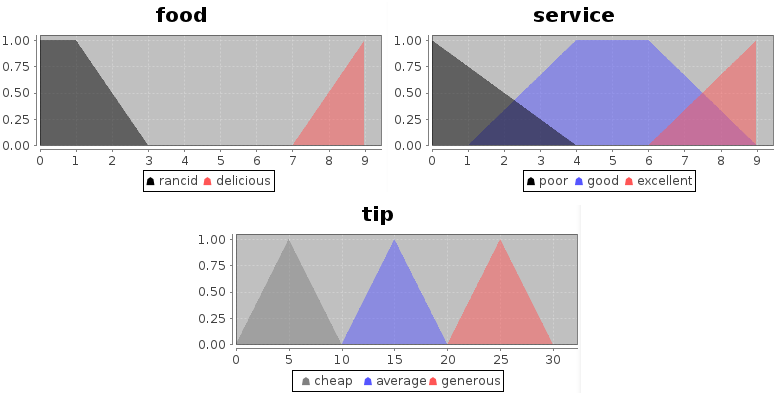
\includegraphics[width=3.15in]{./figs/tipper_MF.png}}
\vspace*{5pt}
\fcaption{Membership functions for tipper example.}\label{f:tipperMf}
\vspace*{10pt}

\begin{scriptsize}
\begin{alltt}
FUNCTION\_BLOCK tipper
VAR\_INPUT
	service, food : REAL;
END\_VAR

VAR\_OUTPUT
	tip : REAL;
END\_VAR

FUZZIFY service
	TERM poor := (0, 1) (4, 0) ;
	TERM good := (1, 0) (4,1) (6,1) (9,0);
	TERM excellent := (6, 0) (9, 1);
END\_FUZZIFY

FUZZIFY food
	TERM rancid := (0, 1) (1, 1) (3,0);
	TERM delicious := (7,0) (9,1);
END\_FUZZIFY

DEFUZZIFY tip
	TERM cheap := (0,0) (5,1) (10,0);
	TERM average := (10,0) (15,1) (20,0);
	TERM generous := (20,0) (25,1) (30,0);
	METHOD : COG;			// Center of Gravity
END\_DEFUZZIFY

RULEBLOCK tipRules
	Rule1:	IF service IS poor OR food IS rancid 
       THEN tip IS cheap;
	Rule2:	IF service IS good THEN tip IS average;
	Rule3:	IF service IS excellent AND food IS delicious 
       THEN tip IS generous;
END\_RULEBLOCK
END\_FUNCTION\_BLOCK
\end{alltt}
\end{scriptsize}


\section{Comparison of fuzzy logic software}
\label{sec:stu}

In this section we present a comparison of non-commercial fuzzy software (Table~\ref{t:comp}). We center our interest on free software because of its important role in the scientific research community~\cite{Sonnenburg07}. This comparison is not intended to be comprehensive or exhaustive. It shows the choices a researcher in the field faces when trying to select a fuzzy logic software package.

\begin{table*}[ht]
{\tiny
\caption{Comparison of open fuzzy logic software packages. Columns describe: Project name (Name), IEC 61131-7 language support (IEC), latest release year (Rel.), main programming language (Lang.), short description from website (Description), number of membership functions supported (MF) and Functionality (notes). Name$^{\ast}$ : package is maintained, compiles correctly, and has extensive functionality.}
\label{t:comp}
\centerline{
\scalebox{1.19}{
\begin{tabular}{@{}|@{\ }l|c|c|l|l|l|l@{\ }|@{}}
\hline
\textbf{Name}		&	\textbf{IEC}	&	\textbf{Rel.}	&	\textbf{Lang.} 	&	\textbf{Description}	&	\textbf{MF}	&	\textbf{Notes}\\
\hline
Akira~\cite{Pezzulo2005}			&	No	&	2007 	&	C++	&	Framework for complex AI agents.	&	4&\\
AwiFuzz~\cite{awifuzz2006}				&	Yes	&	2008 	&	C++	&	Fuzzy logic expert system	&	2	&	Does not compile\\
DotFuzzy~\cite{DotFuzzy2009}		&	No	&	2009 	&	C\#	&	.NET library for fuzzy logic	&	1	&	Specific\\
FFLL~\cite{Zarozinski2002}			&	Yes	&	2003 	&	C++	&	Optimized for speed critical applications.	&	4	&	Does not compile \\
Fispro$^{\ast}$~\cite{Guillaume2011}		&	No	&	2011	&	C++/Java	&	Fuzzy inference design and optimization	&	6	&	\\
FLUtE~\cite{flute2004}			&	No	&	2004 	&	C\#	&	A generic Fuzzy Logic Engine	&	1	&	Beta version \\
FOOL~\cite{Hartwig1996}			&	No	&	2002 	&	C	&	Fuzzy engine	&	5	&	Does not compile\\
FRBS~cite{FRBS2011}			&	No	&	2011	&	C++	&	Fuzzy Rule-Based Systems	&	1	&	Specific\\
Funzy~\cite{Funzy2007}			&	No	&	2007	&	Java	&	Fuzzy Logic reasoning	&	$2^*$	&	Specific\\
Fuzzy Logic Tools$^{\ast}$~\cite{Barragan2011}	&	No	&	2011	&	C++	&	Framework fuzzy control systems,	&	12	&	\\
FuzzyBlackBox~\cite{FuzzyBlackBox2011}		&	No	&	2011	&	-	&	Implementing fuzzy logic	&	-	&	No files released\\
FuzzyClips~\cite{togai2004}		&	No	&	2004	&	C/Lisp	&	Fuzzy logic extension of CLIPS	&	$3 + 2^*$	&	No longer maintained\\
FuzzyJ ToolKit~\cite{Orchard2001}		&	No	&	2006 	&	Java	&	Fuzzy logic extension of JESS	&	15	&	No longer maintained\\
FuzzyPLC$^{\ast}$~\cite{FuzzyPLC2011}	&	Yes	&	2011	&	Java	&	Fuzzy controller for PLC Siemens s226	&	$11 + 14^*$	&	Uses jFuzzyLogic\\
GUAJE$^{\ast}$~\cite{Alonso2011} 		&	No	&	2012	&	Java	&	Development environment 	&		&	Uses FisPro\\
javafuzzylogicctrltool~\cite{javafuzzylogicctrltool2008}	&	No	&	2008	&	Java	&	Framework for fuzzy rules	&	-	&	No files released\\
JFCM~\cite{JFCM2011}			&	No	&	2011	&	Java	&	Fuzzy Cognitive Maps (FCM)	&	-	&	Specific\\
JFuzzinator~\cite{JFuzzinator2010}		&	No	&	2010	&	Java	&	Type-1 Fuzzy logic engine	&	2	&	Specific\\
\textbf{jFuzzyLogic}$^{\ast}$	&	Yes	&	2012 	&	Java	&	FCL and Fuzzy logic API	&	$11 + 14^*$	&	This paper \\
jFuzzyQt$^{\ast}$~\cite{jFuzzyQt2011}	&	Yes	&	2011 	&	C++	&	jFuzzyLogic clone 	&	8	&	\\
libai~\cite{libai2010}			&	No	&	2010 	&	Java 	&	AI library, implements some fuzzy logic 	&	3	&	Specific\\
libFuzzyEngine~\cite{libFuzzyEngine2010}		&	No	&	2010	&	C++	&	Fuzzy Engine for Java	&	1	&	Specific\\
Nefclass~\cite{Nauck1995}			&	No	&	1999	&	C++/Java	&	Neuro-Fuzzy Classification	&	1	&	Specific\\
nxtfuzzylogic~\cite{nxtfuzzylogic2010}		&	No	&	2010	&	Java	&	For Lego Mindstorms NXT	&	1	&	Specific\\
Octave FLT$^{\ast}$~\cite{OctaveFLT2011}	&	No	&	2011	&	Octave	&	Fuzzy logic for Toolkit	&	11	&	\\
XFuzzy3$^{\ast}$~\cite{Baturone2007}	&	No	&	2007	&	Java	&	Development environment	&	6	&	Implements XFL3 specification language\\\hline
\end{tabular}}}}
\end{table*}

We analyze 26 packages (including jFuzzyLogic), mostly from SourceForge or Google-Code, which are considered to be some of the most respectable software repositories. The packages are analyzed in the following categories:
\begin{itemize}
\item \textit{FCL support.} Only four packages ($\sim 17\%$) claim to support IEC 61131-7 specification. Notably, two of them are based on jFuzzyLogic. Only two packages that support FCL are not based on our software. Unfortunately, neither of them seem to be maintained by their developers any longer. Furthermore, one of them has some code taken from jFuzzyLogic.
\item \textit{Programming language.} This is an indicator of code portability. Their languages of choice were mainly Java and C++/C (column \textit{Lang.}). As Java is platform independent it has the advantage of portability. C++ has an advantage in speed and also allows for easier integration in industrial controllers.
\item \textit{Functionality.} Eight packages ($\sim 29\%$) were made for specific purposes, marked as `specific' (column \textit{Notes}, Table \ref{t:comp}). Specific code usually has limited functionality, but it is simpler and has a faster learning curve for the user.
\item \textit{Membership functions}. This is an indicator of how comprehensive and flexible the package is. Specific packages include only one type of membership function (typically trapezoid) and/or one defuzzification method (data not shown). In some cases, arbitrary combinations of membership functions are possible. These packages are marked with an asterisk. For example, `$M+N^*$' means that the software supports $M$ membership functions plus another $N$ which can be arbitrarily combined. 
\item \textit{Latest release.} In nine cases ($\sim 33\%$) there were no released files for the last three years or more (see \textit{Rel.} column in the Table \ref{t:comp}). This may indicate that the package is no longer maintained, and in some cases the web site explicitly mentions this.
\item \textit{Code availability and usability.} Five of the packages ($\sim 21\%$) had no files available, either because the project was no longer maintained or because the project never released any files at all. Whenever the original sites were down, we tried to retrieve the projects from alternative mirrors. In three cases ($\sim 13\%$) the packages did not compile. We performed minimal testing by simply following the instructions, where available, and made no effort to correct any compilation problems. 
\end{itemize}
To summarise, only eight of the software packages ($\sim 33\%$) seemed to be maintained, compiled correctly, and had extensive functionality.  Only two of them (FuzzyPLC and jFuzzyQt) are capable of parsing FCL (IEC 61131-7) files and both are based on jFuzzyLogic. From our point of view users need an open source software which provides the basic programming elements of the standard IEC 61131-7 and is maintained in order to take advantage of the benefits of open source software and standardization. In the next section
we will describe jFuzzyLogic in detail.


\section{JFuzzyLogic \label{sec:jFu}}

JFuzzyLogic's  main goal is to facilitate and accelerate the development of fuzzy systems. We achieve this goal by: i) using standard programming language (FCL) that reduces learning curves; ii) providing a fully functional and complete implementation of FIS; iii) creating API that developers can use or extend; iv) implementing an Eclipse plugin to easily write and test FCL code; v) making the software platform independent; and vi) distributing the software as open source. This allows us to significantly accelerate the development and testing of fuzzy systems in both industrial and academic environments.

In these sections we show how these design and implementation goals were achieved. This should be particularly useful for developers and researchers looking to extend the functionality or use the available API.


\subsection{jFuzzyLogic implementation \label{sec:implement}}

jFuzzyLogic is fully implemented in Java, thus the package is platform independent. ANTLR\cite{parr2007definitive} was used to generate Java code for a lexer and parser based on our FCL grammar definition. This generated parser uses a left to right leftmost derivation recursive strategy, formally know as ``LL(*)".

Using the lexer and parser created by ANTLR we are able to parse FCL files by creating an Abstract Syntax Tree (AST), a well known structure in compiler design. The AST is converted into an Interpreter Syntax Tree (IST), which is capable of performing the required computations. This means that the IST can represent the grammar, like and AST, but is also capable of performing calculations. The parsed FIS can be evaluated by recursively transversing the IST.


\subsection{Membership functions \label{sec:memFun}}


Only two membership functions are defined in the IEC standard: singleton and piece-wise linear. jFuzzyLogic also implements other commonly used membership functions: 
\begin{itemize}
	\item Cosine : $ f(x | \alpha, \beta) = cos[\frac{\pi}{\alpha}(x - \beta)] , \forall x \in [-\alpha, \alpha]$
	\item Difference of sigmoidals: $f(x| \alpha_1, \beta_1, \alpha_2, \beta_2) = s(x,\alpha_1, \beta_1) - s(x,\alpha_2, \beta_2)$, where $s(x,\alpha, \beta) = 1 / [1+e^{-\beta (x-\alpha)}]$
	\item Gaussian : $f(x | \mu, \sigma) = e^{(x-\mu)^2 / 2 \sigma^2}$
	\item Gaussian double : $f(x | \mu_1, \sigma_1,\mu_2, \sigma_2) = $
\[
\left\lbrace \begin{array}{lr}
e^{(x-\mu_1)^2 / 2 \sigma_1^2} & x < \mu_1 \\
1 & \mu_1 \le x \le \mu_2 \\
e^{(x-\mu_2)^2 / 2 \sigma_2^2} & x > \mu_2 \\
\end{array}  \right.
\]
	\item Generalized bell : $f(x |\mu_1,a,b) = \frac{1}{1 + |(x-\mu)/a|^{2b}}$
	\item Sigmoidal : $f(x |\beta, t_0) = \frac{1}{1 + e^{\beta(x-t_0)}}$
	\item Trapezoidal : $f(x | m_{in}, l_{ow}, h_{igh}, m_{ax}) = $
\[
\left\lbrace \begin{array}{lr}
0 & x < m_{in} \\
\frac{x - m_{in} }{l_{ow} - m_{in} } & m_{in} \le x < l_{ow} \\
1 & l_{ow} \le x \le h_{igh} \\
\frac{x - h_{igh} }{m_{ax} - h_{igh} } & h_{igh} < x \le m_{ax} \\
0 & x > m_{ax} \\
\end{array}  \right.
\]
	\item Triangular: $f(x | m_{in}, m_{id}, m_{ax}) = $
\[
\left\lbrace \begin{array}{lr}
0 & x < m_{in} \\
\frac{x -m_{id} }{l_{ow} - m_{id} } & m_{in} \le x \le m_{id} \\
\frac{x - m_{id} }{m_{ax} - m_{id} } & m_{id} < x \le m_{ax} \\
0 & x > m_{ax} \\
\end{array}  \right.
\]
	\item Piece-wise linear : Defined as the union of consecutive points by an affine function.
\end{itemize}

Furthermore, jFuzzyLogic enables arbitrary membership functions to be built by combining mathematical expressions. This is implemented by parsing an Interpreter Syntax Tree (IST) of mathematical expressions. IST is evaluated at running time, thus enabling the inclusion of variables into the expressions. Current implementation allows the use of the following functions:Abs, Cos, Exp, Ln, Log, Modulus, Nop, Pow, Sin, Tan, as well as addition, subtraction, multiplication and division.

It should be noted that, as mentioned in section \ref{sec:Languages}, IEC standard does not define or address the concept of fuzzy partition of a variable.
For this reason, fuzzy partitions are not directly implemented in jFuzzyLogic.
In order to produce a complete partition, we should indicate the membership function for each linguistic term.


\subsection{Aggregation, activation \& accumulation\label{sec:aggActAcc}}

As mentioned in section \ref{sec:Languages}, rules are defined inside the \texttt{RULEBLOCK} statement in an FIS. Each rule  block also specifies aggregation, activation and accumulation methods. All methods defined in the norm are implemented in jFuzzyLogic. It should be noted that we adhere to the definitions of Aggregation, Activation and Accumulation as defined by IEC 61131-7, which may differ from the naming conventions found in other references.

Aggregation methods (sometimes be called ``combination" or ``rule connection methods'') define the t-norms and t-conorms playing the role of AND \& OR operators. Needless to say, each set of operators must satisfy De Morgan's laws. These are shown in Table~\ref{tableAggregation}.
%\begin{table}[ht]
\vspace*{5pt}
\tcap{Aggregation methods.}
\label{tableAggregation}
\centerline{
\scalebox{0.71}{
\begin{tabular}{@{}|l|l|l|@{}}
\hline 
Name & x AND y & x OR y \\ 
\hline 
Min/Max & $min(x,y)$ & $max(x,y)$ \\ 
\hline 
Bdiff/Bsum & $max(0,x+y-1)$ & $min(1,x+y)$ \\ 
\hline 
Prod/PobOr & $x \; y$ & $x + y - x \; y$ \\ 
\hline 
Drastic & if$(x==1) \rightarrow y$  & if$(x==0) \rightarrow y$ \\ 
        & if$(y==1) \rightarrow x$  & if$(y==0) \rightarrow x$ \\ 
        & otherwise $\rightarrow 0$ & otherwise $\rightarrow 1$ \\ 
\hline 
Nil potent & if$( x+y > 1) \rightarrow min(x,y)$  & if$( x+y < 1) \rightarrow max(x,y)$   \\ 
           & otherwise $\rightarrow 0$            & otherwise $\rightarrow 1$ \\ 
\hline 
\end{tabular}}}
\vspace*{10pt}
%\end{table}

Activation method define how rule antecedents modify rule consequents; i.e., once the IF part has been evaluated, how this result is applied to the THEN part of the rule.  
The most common activation operators are Minimum and Product (see Figure~\ref{f:activation}).
Both methods are implemented in jFuzzyLogic.

\vspace*{5pt}
\centerline{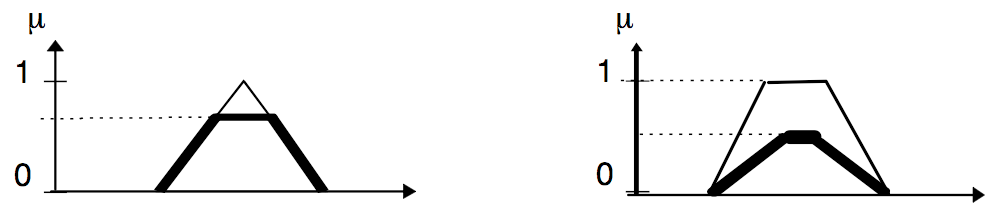
\includegraphics[width=3.1in]{./figs/MaxProd.png}}
\vspace*{3pt}
\fcaption{Activation methods: Min (left) and Prod (right).}\label{f:activation}
\vspace*{5pt}

Finally, the accumulation method defines how the consequents from multiple rules are combined within a Rule Block (see Figure~\ref{f:acumulationOp}).
Accumulation methods implemented by jFuzzyLogic defined in the norm include: 

\begin{itemize}
	\item Maximum : $\alpha_{cc} = max(\alpha_{cc}, \delta)$
	\item Bound sum: $\alpha_{cc} = min(1, \alpha_{cc} + \delta)$
	\item Normalized sum: $\alpha_{cc} = \frac{\alpha_{cc} + \delta}{max(1, \alpha_{cc} + \delta)}$
	\item Probabilistic OR : $\alpha_{cc} =  \alpha_{cc} + \delta -  \alpha_{cc} \; \delta$
\end{itemize}

where $\alpha_{cc}$ is the accumulated value (at point $x$) and $\delta = m(x)$ is the membership function for defuzzification (also at $x$).

\vspace*{5pt}
\centerline{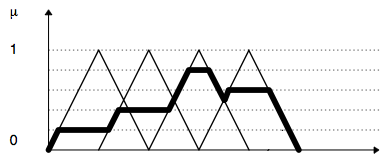
\includegraphics[width=3.1in]{./figs/accumulation.png}}
\vspace*{3pt}
\fcaption{Accumulation method: Combining consequents from multiple rules using ‘Max’ accumulation method.}\label{f:acumulationOp}
\vspace*{5pt}


\subsection{Defuzzification\label{sec:defuzz}}


The last step when evaluating an FIS is defuzzification. The value for each variable is calculated using the selected defuzzification method, which can be:

\begin{itemize}
	\item Center of gravity : $\frac{\int{x \mu(x) dx}}{\int{\mu(x) dx}}$
	\item Center of gravity singleton : $\frac{\sum_{i}{x_i \mu_i}}{\sum_{i}{\mu_i}}$
	\item Center of area : $u \; | \; \int_{-\infty}^{u}{\mu(x) dx} = \int_{u}^{\infty}{\mu(x) dx}$
	\item Rightmost Max : $arg\max_{x}{[ \mu(x) = max(\mu(x)) ] }$
	\item Leftmost Max : $arg\min_{x}{[ \mu(x) = max(\mu(x)) ] }$
	\item Mean max : $mean(x) \; | \; \mu(x) = max(\mu(x)) $
\end{itemize}

When dealing with simple membership functions, such as trapezoidal and piece-wise linear, defuzzicication can be computed easily by applying known mathematical equations.
Although it can be carried out very efficiently, it unfortunately cannot be applyed to arbitrary expressions.

Due to the flexibility in defining membership functions, we use a more general method. We discretize membership functions at a number of points and use a more computational intensive, numerical integration method. The default number of points used for discretization, one thousand, can be adjusted according to the precision-speed trade-off required for a particular application. Inference is performed by evaluating membership functions at these discretization points. In order to perform a discretization, the ``universe" for each variable, has to be estimated. The universe is defined as the range in which the variable has a non-neglectable value. Each membership function and each term is taken into account when calculating a universe for each variable. Once all the rules have been analyzed, the accumulation for each variable is complete. 


\subsection{API extensions \label{sec:ext}}

Some of the extensions and benefits provided by jFuzzyLogic are described in this section.

\textit{Modularity.} The modular design allows us to extend the language and the API easily. It is possible to add custom aggregation, activation or accumulation methods, defuzzifiers, or membership functions by extending the provided object tree (see Figure~\ref{f:tree}). 

\vspace*{7pt}
\centerline{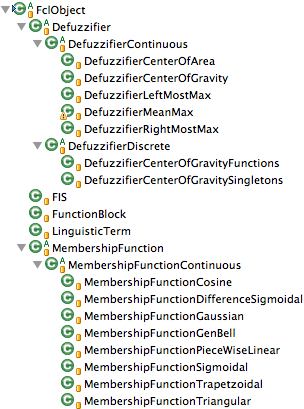
\includegraphics[width=2.5in]{./figs/jFuzzy_object_tree_2.png}}
\vspace*{5pt}
\fcaption{Part of jFuzzyLogic's object tree. Used to provide API extension points.}\label{f:tree}
\vspace*{7pt}

\textit{Dynamic changes.} We have defined an API which supports dynamic changes made to an FIS: i) variables can be used as membership function parameters; ii) rules can be added or deleted from rule blocks, iii) rule weights can be modified; iv) membership functions can use combinations of pre-defined functions. 

\textit{Data Types.} Due to the nature of fuzzy systems and in order to reduce complexity, jFuzzyLogic considers each variable as a \textit{REAL} variable which is mapped to a \textit{double} Java type.

\textit{Execution order.} By default it is assumed that an FIS is composed of only one FB, so evaluating the FIS means evaluating the default FB.  If an FIS has more than one FB, they are evaluated in alphabetical order by FB name. Other execution orders can be implemented by the user, which allows us to define hierarchical controllers easily.


\subsection{Optimization API \label{sec:optim}}


An optimization API was developed in order to automatically fine tune FIS parameters. Our goal was to define a very lightweight and easy to learn API, which was flexible enough to be extended for general purpose usage.

The most common parameters to be optimized are membership functions and rule weights. For instance, if a variable has a fuzzifier term ``\texttt{TERM rancid := trian 0 1 3}", there are three parameters that can be optimized in this membership function (whose initial values are 0, 1 and 3 respectively).  Using the API, we can choose to optimize any subset of them. Similarly, in the rule ``\texttt{IF service IS good THEN tip IS average}" we can optimize the weight of this rule (implicit ``\text{WITH 1.0}" statement). This API consists of the following objects:
\begin{itemize}
	\item \textit{ErrorFunction}: An object that evaluates a Rule Block and calculates the error. Extending ErrorFunction is the bare minimum required to implement an optimization using one of the available optimization methods.
	\item \textit{OptimizationMethod}: An optimization method object is an abstraction of an algorithm. It changes \textit{Parameter} based on the performance measured using an ErrorFunction.
	\item \textit{Parameter}: This class represents a parameter to be optimized. Any change to a parameter, will make the corresponding change to the FIS, thus changing the outcome. There are two basic parameters: ParameterMembershipFunction and ParameterRuleWeight, which allow for changes to membership functions and rule weights respectively. Other parameters could be created in order to, for instance, completely rewrite rules. We plan to extend them in future versions. Most users will not need to extend \textit{Parameter} objects.
\end{itemize}

For most optimization applications, extending only one or two objects is enough (i.e. \textit{ErrorFunction}, and sometimes \textit{OptimizationMethod}). We provide template and demo objects to show how this can be done, all of which are included in our freely available source code.

A few optimization algorithms are implemented, such as gradient descent, partial derivative, and delta algorithm~\cite{hart2001pattern}. As noted above, other algorithms can be easily implemented based on these templates or by directly extending them. In the examples provided it is assumed that error functions can be evaluated anywhere in the input space. This is not a limitation in the API, since we can always develop an optimization algorithm and the corresponding error function that evaluates the FIS on a learning set.

\subsection{Eclipse plugin\label{sec:pluggin}}

Eclipse is one of the most commonly used software development platforms. It allows us to use a specific language development tool by using the Eclipse-plugin framework. We developed a jFuzzyLogic plugin that allows developers to easily and rapidly write FCL code, and test it. Our plugin was developed using Xtext, a well known framework for domain specific languages based on ANTLR.

The plugin supports several features, such as syntax coloring, content assist, validation, program outlines and hyperlinks for variables and linguistic terms, etc. Figure \ref{f:pluginEdit} shows an example of the plugin being used to edit FCL code, where the left panel shows an editor providing syntax coloring while adding content assist at cursor position, and the right panel shows the corresponding code outline. 

\vspace*{7pt}
\centerline{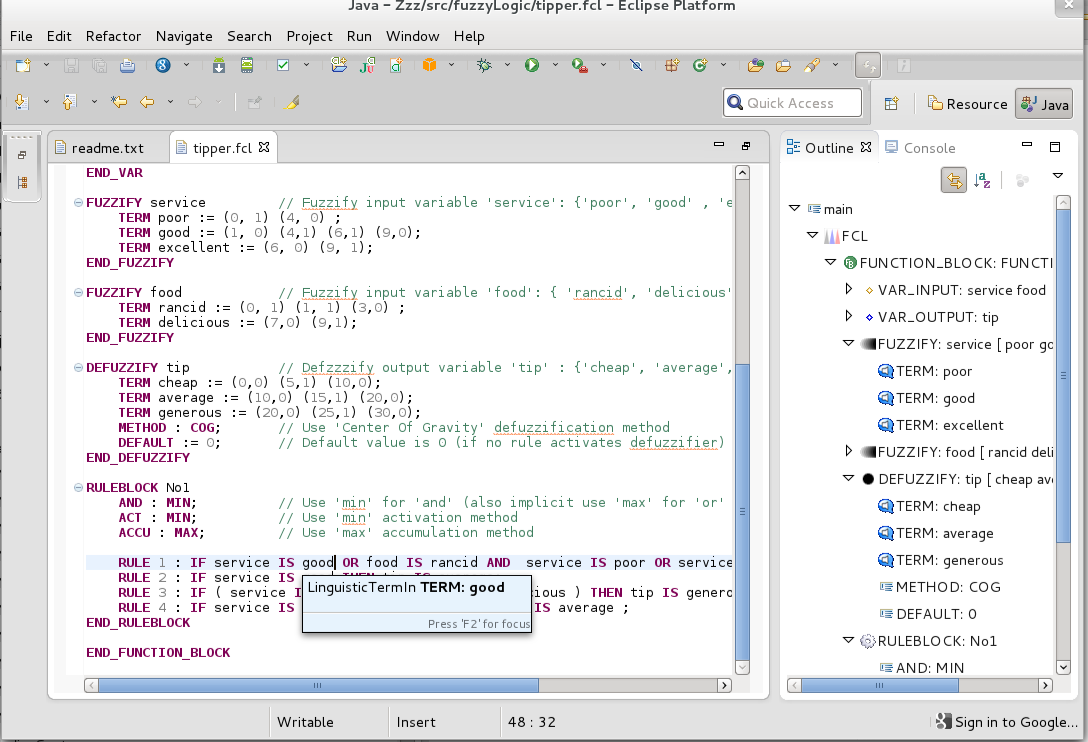
\includegraphics[width=3.15in]{./figs/plugin_edit}}
\vspace*{3pt}
\fcaption{FCL code edited in the Eclipse plugin.}\label{f:pluginEdit}
\vspace*{5pt}

When an FCL program is running, this plugin shows membership functions for all input and output variables. Moreover, the output console shows the FCL code parsed by jFuzzyLogic (Figure \ref{f:pluginRun}) .

\vspace*{7pt}
\centerline{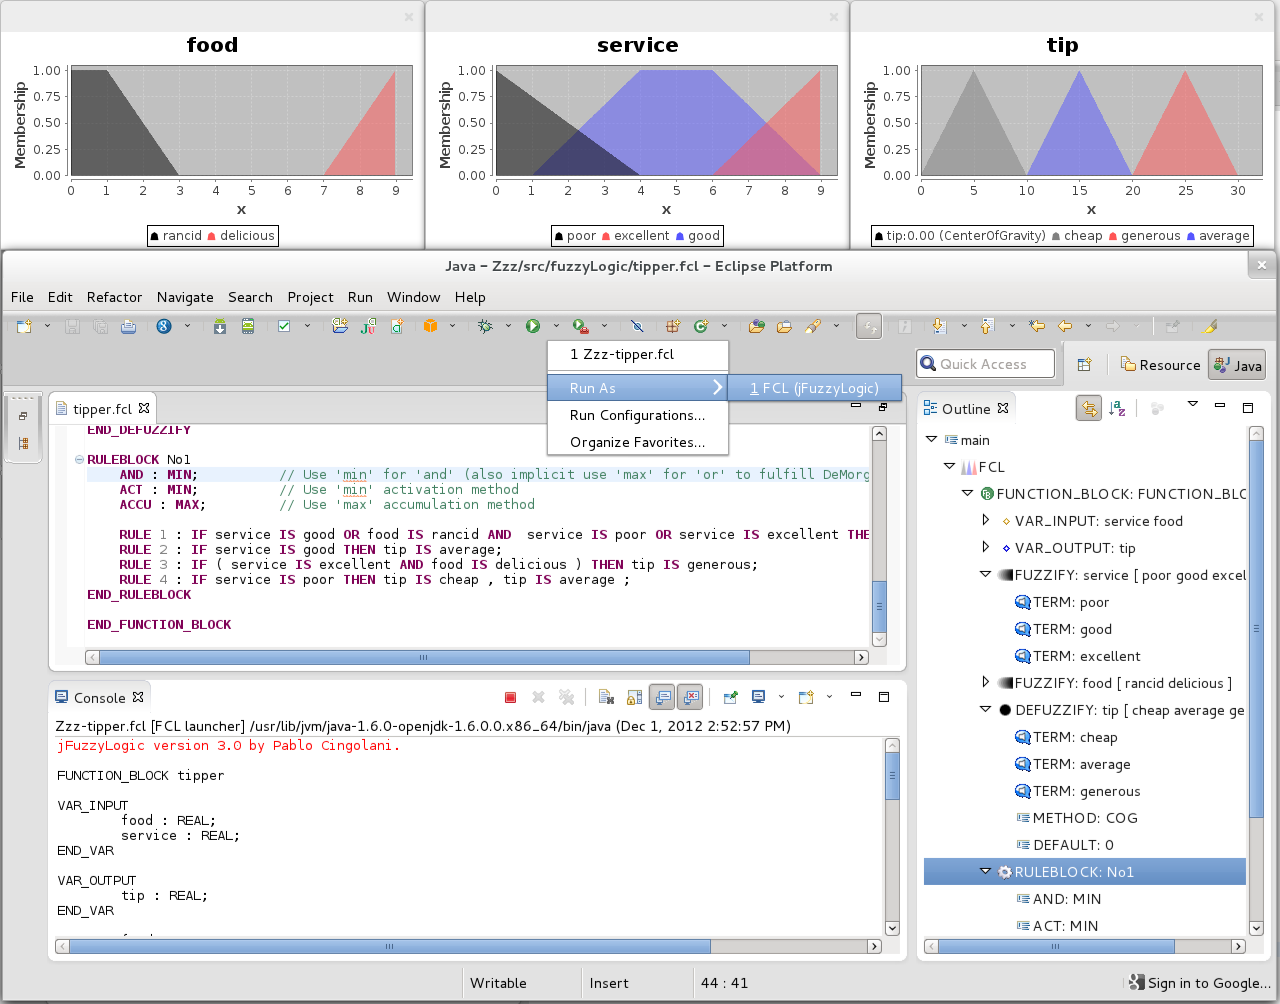
\includegraphics[width=3.15in]{./figs/plugin_run}}
\vspace*{3pt}
\fcaption{Eclipse plugin when an FCL program is running.}\label{f:pluginRun}


\section{A case study}
\label{sec:cas}


In this section we present an example of the creation of a FLC controllers with jFuzzyLogic. This case study is focused on the development of the wall-following robot as explained in \cite{Mucientes2010}. Wall-following behavior is well known in mobile robotics. It is frequently used for the exploration of unknown indoor environments and for the navigation between two points in a map. 

The main requirement of a good wall-following controller is to maintain a suitable distance from the wall that is being followed. The robot should also move as fast as possible, while avoiding sharp movements, making smooth and progressive turns and changes in velocity.


\subsection{Robot fuzzy control system \label{sec:casFuz}}

In our fuzzy control system, the input variables are: i) normalized distances from the robot to the right ($RD$) and left walls ($DQ$); ii) orientation with respect to the wall ($O$); and iii) linear velocity ($V$). 

The output variables in this controller are the normalized linear acceleration ($LA$) and the angular velocity ($AV$). The linguistic partitions are shown in Figure~\ref{f:robotVars}, which are comprised by linguistic terms with uniformly distributed triangular membership functions giving meaning to them.

\vspace*{8pt}
\centerline{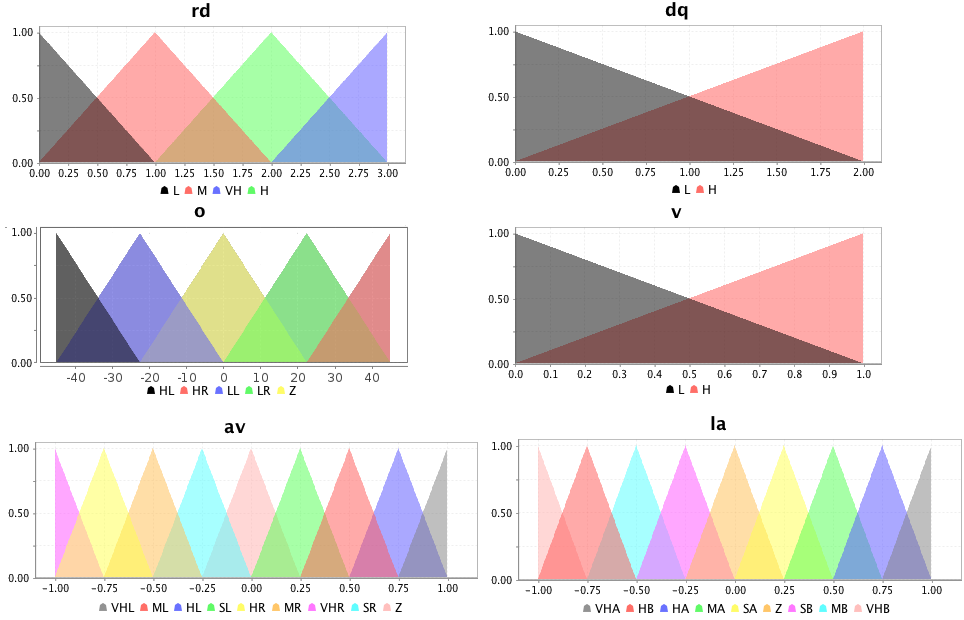
\includegraphics[width=3.15in]{./figs/robot_vars_2.png}}
\vspace*{5pt}
\fcaption{Membership functions for a wall-following robot.}\label{f:robotVars}
\vspace*{8pt}

In order to implement the controller, the first step is to declare the input and output variables and to define the fuzzy sets. Variables are defined in the \textit{VAR\_INPUT} and \textit{VAR\_OUTPUT} sections. Fuzzy sets are defined in \textit{FUZZIFY} blocks for input variables and \textit{DEFUZZIFY} blocks for output variables.

One \textit{FUZZIFY} block is used for each input variable. Each \textit{TERM} line within a \textit{FUZZIFY} block defines a linguistic term and its corresponding membership function.  In this example all membership functions are triangular, so they are defined using the \textit{'trian'} keyword, followed by three parameters defining the left, center and right points.

Output variables define their membership functions within \textit{DEFUZZIFY} blocks. Linguistic terms and membership functions are defined using the \textit{TERM} keyword as previously described for input variables. In this case we also add parameters to select the defuzzification method. The statement \textit{'METHOD : COG'} indicates that we are using 'Center of gravity'. The corresponding FCL code generated for the first step is as follows:

\vspace*{5pt}
\begin{scriptsize}
\begin{alltt}
VAR\_INPUT
	rd : REAL;			// Right distance
	dq : REAL;			// Distance quotient
	o  : REAL;			// Orientation. Note: 'or' is a reserved word
	v  : REAL;			// Velocity
END\_VAR

VAR\_OUTPUT
	la : REAL;			// Linear acceleration
	av : REAL;			// Angular velocity
END\_VAR

FUZZIFY rd
	TERM L  := trian 0 0 1;
	TERM M  := trian 0 1 2;
	TERM H  := trian 1 2 3;
	TERM VH := trian 2 3 3;
END\_FUZZIFY

FUZZIFY dq
	TERM L := trian 0 0 2;
	TERM H := trian 0 2 2;
END\_FUZZIFY

FUZZIFY o
	TERM HL := trian -45 -45 -22.5;
	TERM LL := trian -45 -22.5 0;
	TERM Z  := trian -22.5 0 22.5;
	TERM LR := trian 0 22.5 45;
	TERM HR := trian 22.5 45 45;
END\_FUZZIFY

FUZZIFY v
	TERM L := trian 0 0 1;
	TERM H := trian 0 1 1;
END\_FUZZIFY

DEFUZZIFY la
	TERM VHB := trian -1 -1 -0.75;
	TERM HB  := trian -1 -0.75 -0.5;
	TERM MB  := trian -0.75 -0.5 -0.25;
	TERM SB  := trian -0.5 -0.25 0;
	TERM Z   := trian -0.25 0 0.25;
	TERM SA  := trian 0 0.25 0.5;
	TERM MA  := trian 0.25 0.5 0.75;
	TERM HA  := trian 0.5 0.75 1;
	TERM VHA := trian 0.75 1 1;
	METHOD : COG;			// Center of Gravity
	DEFAULT := 0;
END\_DEFUZZIFY

DEFUZZIFY av
	TERM VHR := trian -1 -1 -0.75;
	TERM HR  := trian -1 -0.75 -0.5;
	TERM MR  := trian -0.75 -0.5 -0.25;
	TERM SR  := trian -0.5 -0.25 0;
	TERM Z   := trian -0.25 0 0.25;
	TERM SL  := trian 0 0.25 0.5;
	TERM ML  := trian 0.25 0.5 0.75;
	TERM HL  := trian 0.5 0.75 1;
	TERM VHL := trian 0.75 1 1;
	METHOD : COG;
	DEFAULT := 0;
END\_DEFUZZIFY
\end{alltt}
\end{scriptsize}
\vspace*{5pt}

These membership functions can be plotted by running jFuzzyLogic with the FCL file generated as argument (e.g. \texttt{java -jar jFuzzyLogic.jar robotWCOR.fcl}). 

The second step is to define the rules used for inference. They are defined in \textit{RULEBLOCK} statements. For the wall-following robot controller, we used 'minimum' connection method (\textit{AND : MIN}), minimum activation method (\textit{ACT : MIN}), and maximum accumulation method (\textit{ACCU : MAX}).  We implemented the RB generated in~\cite{Mucientes2010} by the algorithm WCOR~\cite{Alc06}. Each entry in the RB was converted to a single FCL rule. Within each rule, the antecedent (i.e. the \textit{IF} part) is composed of the input variables connected by \textit{`AND'} operators. Since there is more than one output variable, we can specify multiple consequents (i.e. \textit{THEN} part) separated by semicolons. Finally, we add the desired weight using the \textit{`with'} keyword followed by the weight. This completes the implementation of a controller for a wall-following robot using FCL and jFuzzyLogic. The FLC code generated for the second step is as follows:

\vspace*{4pt}
\begin{scriptsize}
\begin{alltt}
RULEBLOCK rules
AND  : MIN;			// Use 'min' for 'and' (also implicit use 
            //'max' for 'or' to fulfill DeMorgan's Law)
ACT  : MIN;			// Use 'min' activation method
ACCU : MAX;			// Use 'max' accumulation method

RULE 01: IF rd is  L and dq is L and o is LL 
    and v is L THEN la is VHB , av is VHR with 0.4610;
RULE 02: IF rd is  L and dq is L and o is LL 
    and v is H THEN la is VHB , av is VHR with 0.4896;
RULE 03: IF rd is  L and dq is L and o is  Z 
    and v is L THEN la is   Z , av is  MR with 0.6664;
RULE 04: IF rd is  L and dq is L and o is  Z 
    and v is H THEN la is  HB , av is  SR with 0.5435;
RULE 05: IF rd is  L and dq is H and o is LL 
    and v is L THEN la is  MA , av is  HR with 0.7276;
etc;
END\_RULEBLOCK
\end{alltt}
\end{scriptsize}
\vspace*{4pt}

The corresponding whole FCL file for this case study is available for download as one of the examples provided in the jFuzzyLogic package\fnm{c}\fnt{c}{\url{http://jfuzzylogic.sourceforge.net/html/example_java.html}}. The corresponding Java code that uses jFuzzyLogic to run the FCL generated for WCOR is:

\vspace*{4pt}
\begin{scriptsize}
\begin{alltt}
public class TestRobotWCOR \{
  public static void main(String[] args) 
  throws Exception \{
    FIS fis = FIS.load("fcl/robot.fcl", true);
    FunctionBlock fb = fis.getFunctionBlock(null);
    // Set inputs
    fb.setVariable("dp", 1.25);
    fb.setVariable("o", 2.5); 
    fb.setVariable("rd", 0.3); 
    fb.setVariable("v", 0.6);
    // Evaluate
    fb.evaluate(); 
    // Get output
    double la = fb.getVariable("la").getValue());
    double av = fb.getVariable("av").getValue());
  \}
\}
\end{alltt}
\end{scriptsize}

This can also be done using the command line option ``-e", which assigns values in the command line to input variables alphabetically (in this case: ``dp", ``o", ``rd" and ``v") and then evaluates the FIS. Here we show the command, as well as part of the output:

\begin{scriptsize}
\begin{alltt}
java -jar jFuzzyLogic.jar -e robot.fcl 1.2 2.5 0.3 0.6
\vspace*{3pt}
FUNCITON_BLOCK robot
\ 	VAR_INPUT 	        dq = 1.200000
\ 	VAR_INPUT 	         o = 2.500000
\ 	VAR_INPUT 	        rd = 0.300000
\ 	VAR_INPUT 	         v = 0.600000
\ 	VAR_OUTPUT	        av = 0.061952
\ 	VAR_OUTPUT	        la = -0.108399
\   ...(rule activations omitted)
\end{alltt}
\end{scriptsize}

Moreover, this utility also produces plots of membership functions for all variables, as well as the defuzzification areas for the output of all variables. Figure \ref{f:robot_out} shows the defuzzification areas for ``av" and ``la" in light grey.

When evaluation of multiple input values is required, values can be provided as a tab-separated input file using the command line option \texttt{-txt file.txt}. This approach can be easily extended for other data sources, such as databases, online acquisition, etc.

\centerline{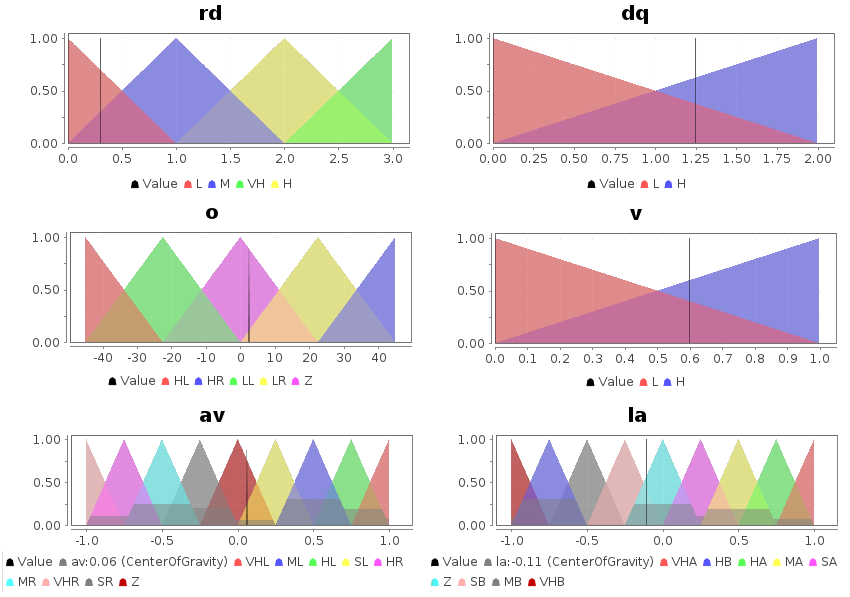
\includegraphics[width=3.15in]{./figs/robot_out2.png}}
\vspace*{5pt}
\fcaption{Membership functions and defuzzification areas (light grey) for \texttt{robots.fcl} example.}\label{f:robot_out}
\vspace*{5pt}


Finally, we can use the jFuzzyLogic Eclipse pluging to see membership functions for all input and output variables and the FCL code parsed by jFuzzyLogic (Figure~\ref{f:pluginFCL}).

\vspace*{5pt}
\centerline{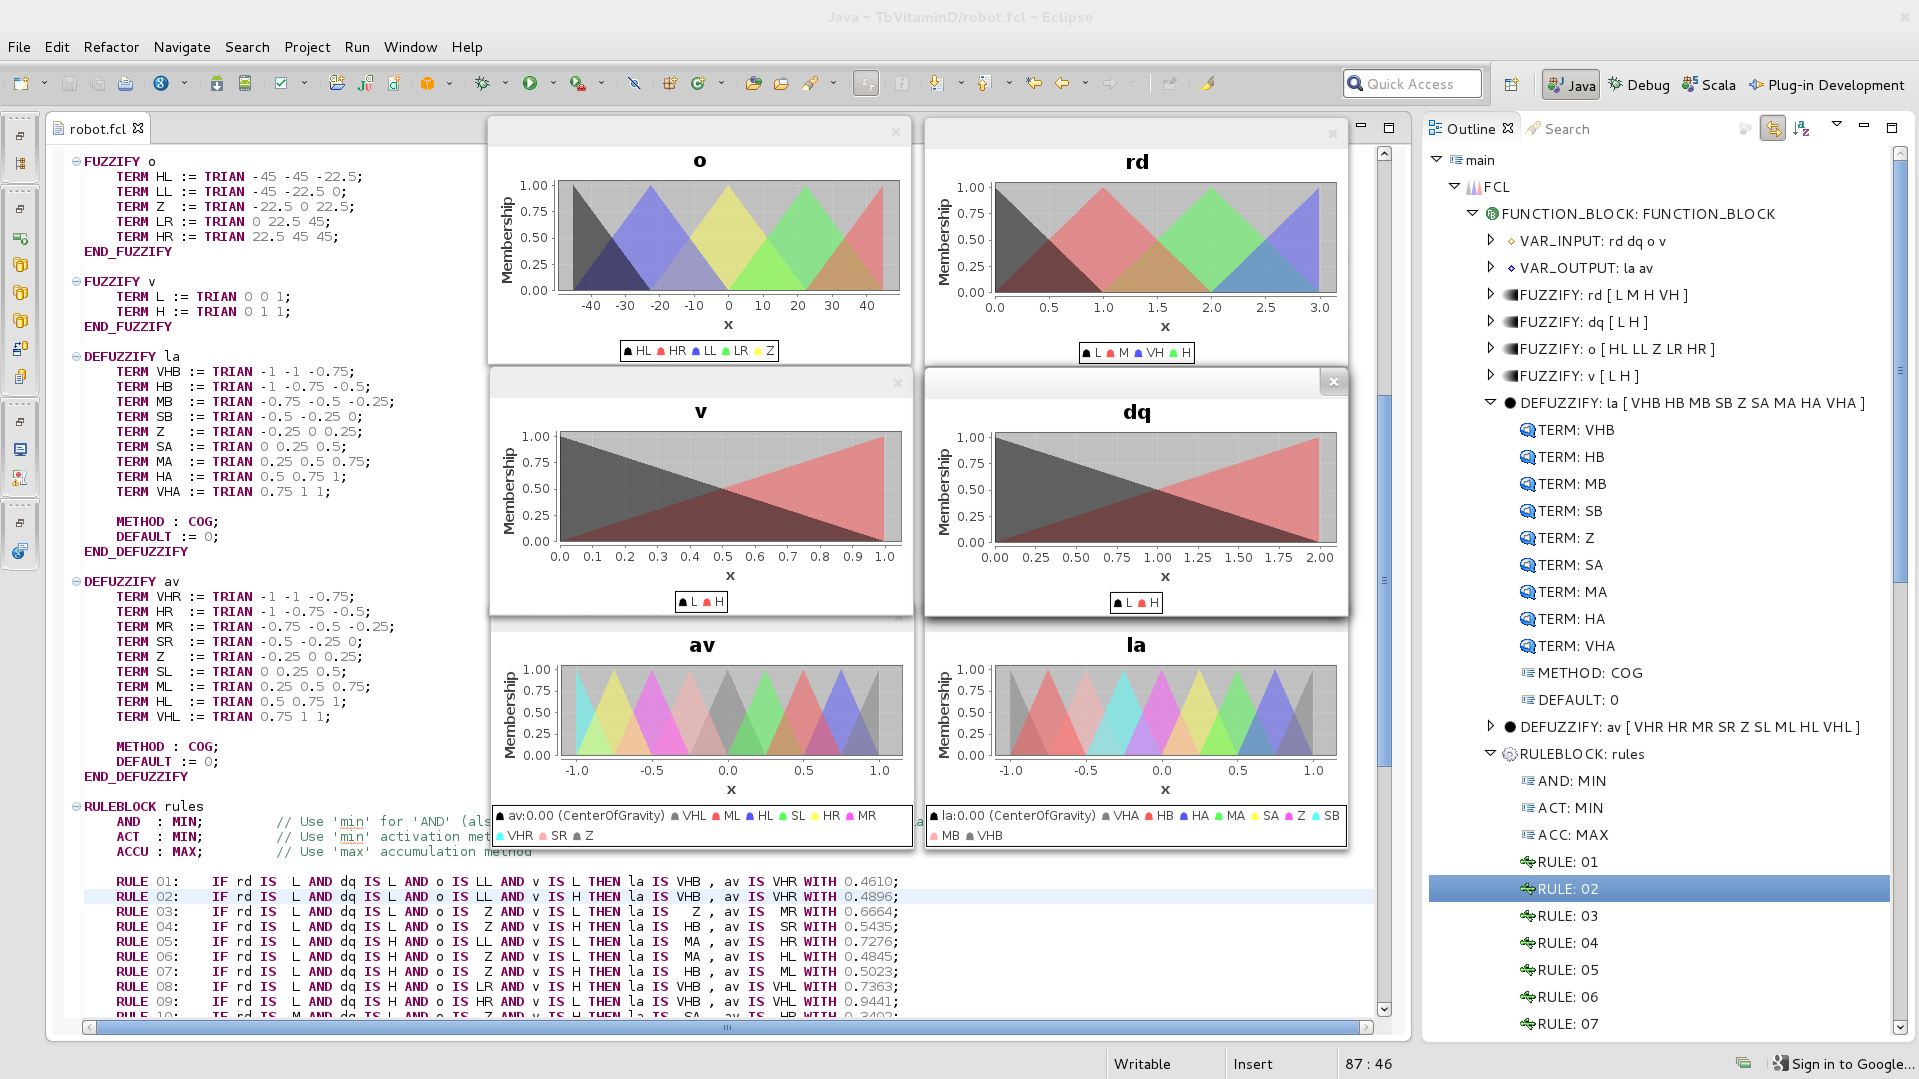
\includegraphics[width=3.15in]{./figs/plugin_optimized_robot.png}}
\vspace*{5pt}
\fcaption{jFuzzyLogic Eclipse pluging with \texttt{robots.fcl} example.}\label{f:pluginFCL}
\vspace*{2pt}
\subsection{Parameter optimization \label{sec:casOpt}}
Continuing our case study, we show an application of the optimization API shown in section \ref{sec:optim}. We apply a parameter optimization algorithm to our FLC for a wall-following robot.

To provide an example, we optimize the membership functions of input variables ``dg" and ``v". Each variable has two \texttt{TRIAN} membership functions, and each triangular membership function has three parameters. Thus, the total number of parameters to optimize is 12. The following code is used to perform the optimization:
\vspace*{4pt}
\begin{scriptsize}
\begin{alltt}
// Load FIS form FCL
FIS fis = FIS.load("robot.fcl");
RuleBlock ruleBlock = fis.getFunctionBlock(null)
                            .getFuzzyRuleBlock(null);
// Get variables
Variable dg = ruleBlock.getVariable("dq");
Variable v = ruleBlock.getVariable("v");

// Add variables to be optimized to parameter list
ArrayList<Parameter> parameterList = new 
                              ArrayList<Parameter>();
parameterList.addAll(Parameter
                  .parametersMembershipFunction(dq));
parameterList.addAll(Parameter
                  .parametersMembershipFunction(v));

// Create optimizaion object and run it
ErrorFunction errFun = new ErrorFunctionRobot
                                    ("training.txt");
optimization = new OptimizationDeltaJump(ruleBlock
                            , errFun, parameterList);
optimization.optimize();
\end{alltt}
\end{scriptsize}
\vspace*{4pt}

An appropriate error function was defined in object ErrorFunctionRobot, which is referenced in the previously shown code. The error function evaluates the controller on a predefined learning set, which consists of 5070 input and output values.

The resulting membership functions from this optimization are shown in Figure \ref{f:optimization_iter_4}. It is easy to see that the optimized membership functions differ significantly from the originally defined ones.

\vspace*{7pt}
\centerline{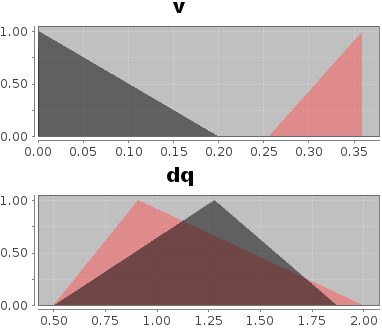
\includegraphics[width=1.6in]{./figs/optimization_iter_4.png}}
\vspace*{2pt}
\fcaption{Membership functions after optimization.}\label{f:optimization_iter_4}
\vspace*{4pt}

The implemented algorithm performs a global optimization. Accordingly, the improvements to the overall RMS error was reduced from $15\%$ in the first iteration, to $3\%$ on the second iteration and only $0.5\%$. on the third one. Further improvements could be obtained by allowing more parameters in the optimization process, at the expense of computational time.
\section{Conclusions}
\label{sec:con}

In this paper, we have described an open source Java library called jFuzzyLogic that allows us to design and to develop FLCs according to the standard IEC 61131-7. jFuzzyLogic offers a fully functional and complete implementation of an FIS and provides an API and Eclipse plugin to easily write and test FCL code. Moreover,  this library relieves researchers of much technical work and enables researchers with little knowledge of fuzzy logic control to apply FLCs to their control applications.

We have shown a case study to illustrate the use of jFuzzyLogic. In this case, we developed a FLC for wall-following behavior in a robot. The example shows how jFuzzyLogic can be used to easily implement and to run a FLC. Moreover, we have shown how we can use jFuzzyLogic to tune a FLC.

The jFuzzyLogic software package is continuously being updated and improved. 
Future work includes: 
	i) using defuzzifier analytic solutions wherever possible (e.g. FIS consisting exclusively of trapezoidal and triangular sets), as it would considerably speed-up processing; 
	ii) adding FIS constraints and developing ways to include them as part of the language extensions; and
	iii) at the moment, we are developing an implementation of an FCL to C/C++ compiler, allowing easy implementation of embedded control systems.

\vspace{-0.19cm}
\section*{Acknowledgments}

jFuzzyLogic was designed and developed by P. Cingolani. He is supported in part by McGill Uninversity, Genome Quebec. J. Alcala-Fdez is supported by the Spanish Ministry of Education and Science under Grant TIN2011-28488 and the Andalusian Government under Grant P10-TIC-6858. We would like to thank R. Sladek and M. Blanchette for their comments. Special thanks to P.J. Leonard for his contributions to the project.

\vspace{-0.19cm}
\section*{References}
% \bibliographystyle{unsrt}
% \bibliography{CingolaniAlcala-Fdez-IJCIS2012}
\begin{thebibliography}{10}

\bibitem{Lee90}
C.C. Lee,
\newblock ``Fuzzy logic in control systems: Fuzzy logic controller parts i and
  ii,"
\newblock {\it IEEE Transactions on Systems, Man, and Cybernetics},
  {\bf 20}, 404--435 (1990).

\bibitem{DHR93}
H.~Hellendoorn D.~Driankov and M.~Reinfrank,
\newblock ``An Introduction to Fuzzy Control,"
\newblock {\it Springer-Verlag} (1993).

\bibitem{Bon94}
P.P. Bonissone, 
\newblock ``Fuzzy logic controllers: An industrial reality," {\it In Computational Intelligence: Imitating Life, IEEE Press}, 316--327 (1994).

\bibitem{EH2010}
B.E. Eskridge and D.F. Hougen,
\newblock ``Extending adaptive fuzzy behavior hierarchies to multiple levels of
  composite behaviors," {\it Robotics And Autonomous Systems}, {\bf 58:9}, 1076--1084 (2010).

\bibitem{JCh2011}
Ch.-F. Juang and Y.-Ch. Chang,
\newblock ``Evolutionary-group-based particle-swarm-optimized fuzzy controller
  with application to mobile-robot navigation in unknown environments," {\it IEEE Transactions on Fuzzy Systems}, {\bf 19:2}, 379--392 (2011).

\bibitem{Alc09}
R.~Alcal{\'a}, J.~Alcal{\'a}-Fdez, M.J. Gacto, and F.~Herrera,
\newblock ``Improving fuzzy logic controllers obtained by experts: a case study
  in HVAC systems," {\it Applied Intelligence}, {\bf 31:1}, 15--30 (2009).

\bibitem{Cho11}
E.~Cho, M.~Ha, S.~Chang, and Y.~Hwang,
\newblock ``Variable fuzzy control for heat pump operation," {\it Journal of Mechanical Science and Technology}, {\bf 25:1}, 201--208
  (2011).

\bibitem{Cha12}
F.~Ch{\'a}vez, F.~Fern{\'a}ndez, R.~Alcal{\'a}, J.~Alcal{\'a}-Fdez, G.~Olague,
  and F.~Herrera,
\newblock ``Hybrid laser pointer detection algorithm based on template matching
  and fuzzy rule-based systems for domotic control in real home enviroments," {\it Applied Intelligence}, {\bf 36:2}, 407--423 (2012).

\bibitem{AL05}
G.~Acampora and V.~Loia,
\newblock ``Fuzzy control interoperability and scalability for adaptive domotic
  framework," {\it IEEE Transactions on Industrial Informatics}, {\bf 1:2}, 97 -- 111
  (2005).

\bibitem{Otero2008}
J.~Otero, L.~S\'anchez, and J.~Alcal\'a-Fdez,
\newblock ``Fuzzy-genetic optimization of the parameters of a low cost system for
  the optical measurement of several dimensions of vehicles," {\it Soft Computing}, {\bf 12:8}, 751--764 (2008).

\bibitem{Demir12}
O.~Demir, I.~Keskin, and S.~Cetin,
\newblock ``Modeling and control of a nonlinear half-vehicle suspension system: A
  hybrid fuzzy logic approach," {\it Nonlinear Dynamics}, {\bf 67:3}, 2139--2151 (2012).

\bibitem{ZG2012}
Y.~Zhao and H.~Gao,
\newblock ``Fuzzy-model-based control of an overhead crane with input delay and
  actuator saturation," {\it IEEE Transactions on Fuzzy Systems}, {\bf 20:1}, 181 --186 (2012).

\bibitem{Sonnenburg07}
S.~Sonnenburg, M.L. Braun, Ch.S. Ong, S.~Bengio, L.~Bottou, G.~Holmes,
  Y.~LeCun, K.-R. Muller, F.~Pereira, C.E. Rasmussen, G.~Ratsch, B.~Scholkopf,
  A.~Smola, P.~Vincent, J.~Weston, and R.~Williamson,
\newblock ``The need for open source software in machine learning," {\it Journal of Machine Learning Research}, {\bf 8}, 2443--2466 (2007).

\bibitem{IEC}
``International Electrotechnical Commission technical committee industrial
  process measurement and control. IEC 61131 - Programmable Controllers,"
\newblock {\it IEC} (2000).

\bibitem{Mamdani1974}
E.H. Mamdani,
\newblock ``Applications of fuzzy algorithms for control a simple dynamic plant,"
\newblock {\it Proceedings of the Institution of Electrical Engineers},
  {\bf 121:12}, 1585--1588 (1974).

\bibitem{MA1975}
E.H. Mamdani and S.~Assilian,
\newblock ``An experiment in linguistic synthesis with a fuzzy logic controller," {\it International Journal of Man-Machine Studies}, {\bf 7}, 1--13 (1975).

\bibitem{Zadeh1965}
L.A. Zadeh,
\newblock ``Fuzzy sets," {\it Information and Control}, {\bf 8}, 338--353 (1965).

\bibitem{Wan94}
L.X. Wang,
\newblock ``Adaptive Fuzzy Systems and Control. Design and Stability
  Analysis," {\it Prentice-Hall} (1994).

\bibitem{CHP97}
O.~Cord\'on, F.~Herrera, and A.~Peregr\'in,
\newblock ``Applicability of the fuzzy operators in the design of fuzzy logic
  controllers," {\it Fuzzy Sets and Systems}, {\bf 86}, 15--41 (1997).

\bibitem{Kamen1999}
E.W. Kamen,
\newblock ``Ladder logic diagrams and plc implementations," {\it In Industrial Controls and Manufacturing, Academic Press}, 141--164 (1999).

\bibitem{Reisig1991}
W.~Reisig,
\newblock ``Petri nets and algebraic specifications," {\it Theoretical Computer Science}, {\bf 80:1}, 1--34 (1991).

\bibitem{Pezzulo2005}
G.~Pezzulo and G.~Calvi,
\newblock ``Designing and implementing mabs in akira,"
\newblock {\it In P.~Davidsson, B.~Logan, and K.~Takadama, editors, Multi-Agent
  and Multi-Agent-Based Simulation, Lecture Notes in Computer Science, Springer Berlin Heidelberg}, {\bf 3415}, 49--64 (2005), 
\newblock \url{http://www.akira-project.org/}.

\bibitem{awifuzz2006}
``Awifuzz - fuzzy logic control system,"
\newblock \url{http://awifuzz.sourceforge.net/} (2006).

\bibitem{DotFuzzy2009}
``Dotfuzzy," \url{http://www.havana7.com/dotfuzzy/} (2009).

\bibitem{Zarozinski2002}
M.~Zarozinski,
\newblock ``An open source fuzzy logic library,"
\newblock {\it In AI Game Programming Wisdom, Charles River Media}, 90--103 (2002), 
\newblock \url{http://ffll.sourceforge.net/}.

\bibitem{Guillaume2011}
Serge Guillaume and Brigitte Charnomordic,
\newblock ``Learning interpretable fuzzy inference systems with fispro,"
\newblock {\it International Journal of Information Sciences},
  {\bf 181:20}, 4409--4427 (2011), 
\newblock \url{http://www.inra.fr/mia/M/fispro/}.

\bibitem{flute2004}
``Flute: Fuzzy logic ultimate engine,"
\newblock \url{http://flute.sourceforge.net/} (2004).

\bibitem{Hartwig1996}
Ronald Hartwig, Carsten Labinsky, Sven Nordhoff, Bernd Landorff, Peter Jensch,
  and Joerg Schwanke,
\newblock ``Free fuzzy logic system design tool: Fool," {\it In 4th European congress on intelligent techniques and soft computing (EUFIT)}, {\bf 3}, 2274--2277 (1996), \url{http://rhaug.de/fool/}.

\bibitem{Funzy2007}
``Funzy," \url{http://code.google.com/p/funzy/} (2007).

\bibitem{Barragan2011}
A.~Barrag\'an and J.M. And\'ujar,
\newblock ``Fuzzy Logic Tools. Reference Manual v1.0," {\it Universidad de Huelva publicaciones} (2011), \url{http://uhu.es/antonio.barragan/category/temas/fuzzy-logic-tools}.

\bibitem{FuzzyBlackBox2011}
``Fuzzyblackbox," \url{http://fuzzyblackbox.sourceforge.net/} (2011).

\bibitem{togai2004}
Togai InfraLogic,
\newblock ``Fuzzyclips," \url{http://www.ortech-engr.com/fuzzy/fzyclips.html} (2004).

\bibitem{Orchard2001}
R.A. Orchard,
\newblock ``Fuzzy reasoning in jess: The fuzzyj toolkit and fuzzyjess," {\it 3rd International Conference on Enterprise Information Systems (ICEIS)}, {\bf 2}, 533--542 (2001), \url{http://ai.iit.nrc.ca/IR_public/fuzzy/fuzzyJDocs/index.html}.

\bibitem{FuzzyPLC2011}
``Fuzzyplc," \url{http://fuzzyplc.sourceforge.net/} (2011).

\bibitem{Alonso2011}
J.M. Alonso and L.~Magdalena,
\newblock ``Generating understandable and accurate fuzzy rule-based systems in a
  java environment," {\it 9th International Workshop on Fuzzy Logic and Applications
  (WILF), Lecture Notes in Artificial Intelligence, Springer-Verlag}, {\bf 6857}, 212--219 (2011),  \url{http://sourceforge.net/p/guajefuzzy/wiki/Home/}.

\bibitem{javafuzzylogicctrltool2008}
``javafuzzylogicctrltool," \url{http://code.google.com/p/javafuzzylogicctrltool/} (2008).

\bibitem{JFCM2011}
``Java fuzzy cognitive maps," \url{http://jfcm.megadix.it/} (2011).

\bibitem{JFuzzinator2010}
``Jfuzzinator," \url{http://jfuzzinator.sourceforge.net/} (2010).

\bibitem{jFuzzyQt2011}
``jfuzzyqt - C++ fuzzy logic library," \url{http://jfuzzyqt.sourceforge.net/} (2011).

\bibitem{libai2010}
``libai," \url{http://libai.sourceforge.net/} (2010).

\bibitem{libFuzzyEngine2010}
``libfuzzyengine," \url{http://libfuzzyengine.git.sourceforge.net/git/gitweb-index.cgi} (2010).

\bibitem{Nauck1995}
Detlef Nauck and Rudolf Kruse,
\newblock ``Nefclass - a neuro-fuzzy approach for the classification of data," {\it ACM Symposium on Applied Computing}, 461--465 (1995), \url{http://fuzzy.cs.uni-magdeburg.de/nefclass/}.

\bibitem{nxtfuzzylogic2010}
``nxtfuzzylogic," \url{http://code.google.com/p/nxtfuzzylogic/} (2010).

\bibitem{OctaveFLT2011}
``Fuzzy logic toolkit for octave,"
\newblock
  \url{http://pdb.finkproject.org/pdb/package.php/fuzzy-logic-toolkit-oct324} (2011).

\bibitem{Baturone2007}
I.~Baturone, F.J. Moreno-Velo, S.~S\'anchez-Solano, A.~Barriga, P.~Brox,
  A.~Gersnoviez, and M.~Brox,
\newblock ``Using xfuzzy environment for the whole design of fuzzy systems," {\it IEEE International Conference on Fuzzy Systems}, 1--6 (2007), \url{http://www2.imse-cnm.csic.es/Xfuzzy/Xfuzzy_3.0/index.html}.

\bibitem{parr2007definitive}
T.~Parr, ``The definitive ANTLR reference: building domain-specific languages" (2007).

\bibitem{hart2001pattern}
{R.O.} Duda, {P.E.} Hart, and {D.G.} Stork,
\newblock ``Pattern classification," {\it John Willey \& Sons} (2001).

\bibitem{Mucientes2010}
M.~Mucientes, J.~Alcal\'a-Fdez, R.~Alcal\'a, and J.~Casillas,
\newblock ``A case study for learning behaviors in mobile robotics by evolutionary fuzzy systems," {\it Expert Systems with Applications}, {\bf 37:2}, 1471--1493 (2010).

\bibitem{Alc06}
R.~Alcal{\'a}, J.~Alcal{\'a}-Fdez, J.~Casillas, O.~Cord{\'o}n, and F.~Herrera,
\newblock ``Hybrid learning models to get the interpretability-accuracy trade-off
  in fuzzy modelling," {\it Soft Computing}, {\bf 10:9}, 717--734 (2006).

\end{thebibliography}


\end{multicols}
\end{document}
